

\section{Procesos de nacimiento y muerte}

Para analizar este tipo de procesos definimos el número de personas presentes en el sistema en el tiempo $t$ como el estado del sistema en ese tiempo $t$. Consideramos $p_{ij}^n$ la probabilidad de que, habiendo $i$ personas en el sistema, después de $n$ pasos halla $j$ personas. Hemos visto anteriormente que cuando $n$ es suficientemente grande esas probabilidades se estabilizan en $\pi_j$. Diremos que $p_{ij}^n$ tiene un \textbf{comportamiento transitorio} si $p_{ij}^n$ aún no ha alcanzado el estado estable. Por ahora, supondremos que el estado estable ya se alcanzó y trabajaremos con $\pi_j$.

\subsection{Leyes de movimiento}

Sea $\lbrace X(t), t\geq 0 \rbrace$ el proceso de tiempo continuo que indica el número de personas en el sistema en el tiempo $t$ y $S=\lbrace 0,1,2,.,j,..\rbrace$ el espacio de estados. Supongamos que para cierto $t$, $X(t)=j$. Los procesos de nacimiento-muerte se rigen por tres leyes básicas:

\begin{enumerate}
	
	\item $P$(1 nacimiento entre $(t, t+h)$)=$\lambda_j h +o(h)$.\\
	El estado se incrementa en 1, esto es, $X(t+h)=j+1$.
	$\lambda_j$ es la tasa de nacimiento en el estado $j$ (equivaldría a una llegada).
	
	\item $P$(1 muerte entre $(t, t+h)$)=$\mu_j h +o(h)$.\\
	El estado se disminuye en 1, esto es, $X(t+h)=j-1$.
	$\mu_j$ es la tasa de muerte en el estado $j$ (equivaldría a una salida).
	
	\item Los nacimientos y muertes son independientes.
	
	
\end{enumerate} 

\begin{figure}[h]
	\centering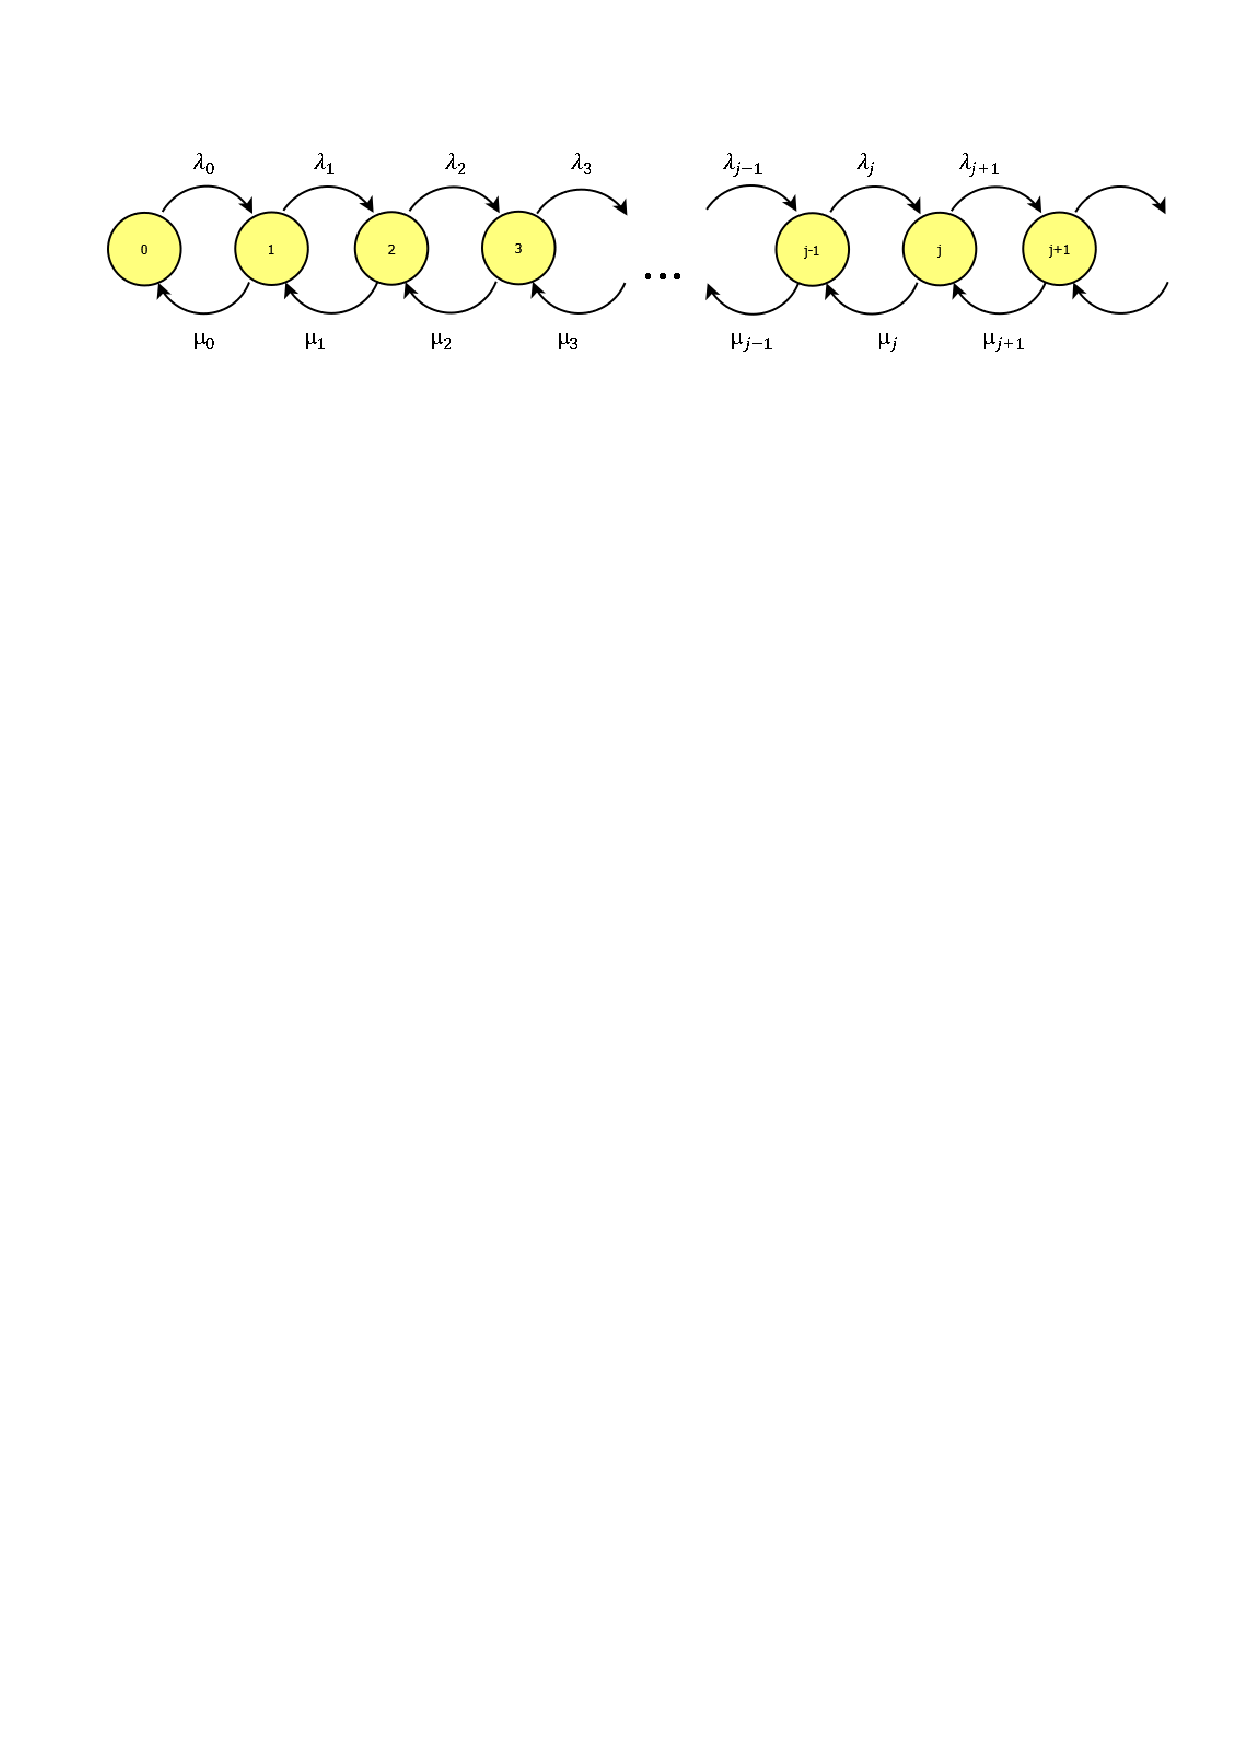
\includegraphics[trim = 10mm 220mm 10mm 25mm, clip,width=0.9\linewidth]{diagramatasa}
	\caption{Diagrama de tasas}
\end{figure}

Consideremos que tanto los nacimientos como las muertes siguen distribuciones exponenciales de parámetros $\lambda$ y $\mu $ respectivamente. \\
Por la carencia de memoria de la distribución exponencial, la probabilidad de que un nacimiento ocurra durante $(t,t+h)$ es de:

$$
\int_{0}^{h}  \lambda \, e^{-\lambda t} \, dt = 1-e^{-\lambda h}=1-(1-\lambda h + o(h))=\lambda h + o(h)
$$

Del mismo modo, la probabilidad de que ocurra una muerte durante $(t,t+h)$ es de:

$$
\int_{0}^{h}  \mu \, e^{-\mu t} \, dt = 1-e^{-\mu h}=1-(1-\mu h + o(h))=\mu h + o(h)
$$ 

Es posible desarrollar un modelo modificado de nacimiento-muerte con los tiempos de llegada y servicio siguiendo distribuciones Erlang.

\subsection{Cálculo de $\pi_j$}

Para determinar las $\pi_j$ relacionamos $p_{ij}(t)$ con $p_{ij}(t+h)$ para $h$ pequeña. 

Es fácil ver que

\begin{equation*}
\begin{split}
p_{ij}(t+h)= p_{i,j-1}(t)P(\textrm{1 nacimiento en } (t,t+h))+\\
+ p_{i,j+1}(t)P(\textrm{1 muerte en }(t,t+h))+\\
+ p_{ij}(t)P(\textrm{ningún nacimiento ni muerte en }(t,t+h))
\end{split}
\end{equation*}

Esto es


\begin{equation}
\begin{split}
p_{ij}(t+h)= p_{i,j-1}(t)(\lambda_{j-1}h + o(h))+\\
+ p_{i,j+1}(t)(\mu_{j+1}h + o(h))+\\
+ p_{ij}(t)(1-\lambda_{j}h - \mu_{j}h + o(h) )
\end{split}
\end{equation}



Reagrupando:

\begin{equation*}
p_{ij}(t+h) = p_{ij}(t) + h(\lambda_{j-1} p_{i,j-1}(t) + \mu_{j+1}  p_{i,j+1}(t) - \lambda_j  p_{ij} - \mu_{j} p_{ij}(t) + o(h))
\end{equation*}



Restando a ambos lados de la igualdad $p_{ij}(t)$ y dividiendo entre $h$ tenemos:


\begin{equation*}
\frac{p_{ij}(t+h)-p_{ij}(t)}{h}=\lambda_{j-1} p_{i,j-1}(t) + \mu_{j+1}  p_{i,j+1}(t) - \lambda_j  p_{ij}(t) - \mu_{j} p_{ij}(t) + o(h)
\end{equation*}

Tomando límite de $h$ tendiendo a 0 nos queda:


\begin{equation*}
p_{ij}'(t)= \lambda_{j-1} p_{i,j-1}(t) + \mu_{j+1}  p_{i,j+1}(t) - \lambda_j  p_{ij}(t) - \mu_{j} p_{ij}(t)
\end{equation*}

Para $t$ grande y cualquier estado inicial $i$, $p_{ij}(t)=\pi_{j}$ constante. Por lo tanto, $p_{ij}(t)'=0$. Sustituyendo todos las probabilidades de estado estable en la ecuación, se tiene:

\begin{equation*}
\lambda_{j-1} \pi_{j-1} + \mu_{j+1}  \pi{j+1} - \lambda_j  \pi_{j} - \mu_{j} \pi_{j}=0
\end{equation*}

\begin{equation}
\lambda_{j-1} \pi_{j-1} + \mu_{j+1}  \pi_{j+1} = \pi_j(\lambda_j + \mu_j) \qquad (j= 1,2,...) \label{eq1}
\end{equation}


Para $j=0$, tenemos:

\begin{equation}
\mu_1 \pi_1 = \pi_0 \lambda_0
\label{eq2}
\end{equation}

Las ecuaciones ($\ref{eq1}$) y ($\ref{eq2}$) se llaman \textbf{ecuaciones de balance de flujo} para un proceso de nacimiento-muerte.\\

\textbf{Solución de las ecuaciones de balance de flujo en un proceso de nacimiento-muerte:}\\

Primero, expresamos todas las $\pi_j$ en función del término $\pi_0$.\\

De (\ref{eq2}) obtenemos

\begin{equation}
\pi_1=\frac{\pi_0 \lambda_0}{\mu_1}
\label{eq3}
\end{equation}

Al sustituir (\ref{eq3}) en (\ref{eq1}) para $j=1$ y despejando $\pi_2$ tenemos

\begin{equation}
\pi_2=\frac{\pi_0(\lambda_0 \lambda_1)}{\mu_1 \mu_2}
\label{eq4}
\end{equation}

Procediendo análogamente para $j=3,4,..$ se tiene que

\begin{equation}
\pi_j=\pi_0 c_j
\label{eq5}
\end{equation}

donde $c_j=\dfrac{\lambda_0 \lambda_1 \cdots \lambda_{j-1}}{\mu_1 \mu_2 \cdots \mu_j}$.\\

Como debemos estar en algún estado para cualquier tiempo $t$:

\begin{equation}
\sum_{j=0}^{\infty}\pi_j=1 
\label{eq6}
\end{equation}

Sustituyendo ($\ref{eq5}$) en (7) se llega a

\begin{equation*}
\pi_0 \left( 1+\sum_{j=1}^{\infty} c_j \right) = 1 
\end{equation*}

Despejando $\pi_0$, si la serie es convergente:

\begin{equation}
\pi_0=\dfrac{1}{1+\sum_{j=1}^{\infty} c_j}
\label{eq6}
\end{equation}

Por lo tanto, una vez que calculemos $\pi_0$ utilizando $(6)$ podremos calcular cualquier $\pi_j$ mientras estemos en estado de equilibrio. \\
Se puede demostrar que si:
$$
\sum_{j=1}^{\infty} c_j = \infty $$
Entonces el sistema no existe una distribución de estado estable.